\documentclass[12pt,notes]{beamer}
 
\usetheme{FHWN}
\usepackage[utf8]{inputenc}
\usepackage{includes/masterthesis-vars}
\usepackage[UKenglish]{isodate}

\usepackage[group-separator={,}]{siunitx}
\usepackage{supertabular}
\usepackage[nomain,acronym,toc,shortcuts]{glossaries}

\usepackage[backend=bibtex,style=numeric,sorting=anyvt,natbib=true]{biblatex}
\addbibresource{thesis-includes/part00-preamble-mainreferences.bib}  %Imports bibliography file
\addbibresource{thesis-includes/part00-preamble-tweetreferences.bib} %Imports bibliography file

% the following section is from: https://tex.stackexchange.com/questions/97615/article-style-bibliography-in-beamer-class

% make bibliography entries smaller
\renewcommand\bibfont{\scriptsize}
% If you have more than one page of references, you want to tell beamer
% to put the continuation section label from the second slide onwards
\setbeamertemplate{frametitle continuation}[from second]
% and kill the abominable icon
%\setbeamertemplate{bibliography item}{}
% Now get rid of all the colours
\setbeamercolor*{bibliography entry title}{fg=black}
\setbeamercolor*{bibliography entry author}{fg=black}
\setbeamercolor*{bibliography entry location}{fg=black}
\setbeamercolor*{bibliography entry note}{fg=black}

\newcolumntype{!}{>{\global\let\currentrowstyle\relax}}
\newcolumntype{^}{>{\currentrowstyle}}
\newcommand{\rowstyle}[1]{\gdef\currentrowstyle{#1}%
  #1\ignorespaces
}

\AtBeginSection[]{
  \frame{\tableofcontents[currentsection]}
  % \begin{frame}
  % \vfill
  % \centering
  % \begin{beamercolorbox}[sep=8pt,center,shadow=true,rounded=false]{title}
  %   \usebeamerfont{title}\insertsectionhead\par%
  % \end{beamercolorbox}
  % \vfill
  % \end{frame}
}

\institute{Matriculation No.: \matriculationNumber}
\date{\printdate{2019-06-19}}

%!TEX root = ../thesis.tex

\newacronym{EMH}{EMH}{Efficient Market Hypothesis}
\newacronym{ME}{ME}{Maximum Entropy}
\newacronym{NB}{NB}{Naive Bayes}
\newacronym{NLP}{NLP}{Natural Language Processing}
\newacronym{SVM}{SVM}{Support Vector Machines}
\newacronym{TP}{TP}{True Positive}
\newacronym{TN}{TN}{True Negative}
\newacronym{FP}{FP}{False Positive}
\newacronym{FN}{FN}{False Negative}
\newacronym{bow}{bow}{bag of words}
\newacronym{API}{API}{Application Programming Interface}
\newacronym{GB}{GB}{Giga Bytes}
\newacronym{RegEx}{RegEx}{Regular Expression}
\newacronym{TF-IDF}{TF-IDF}{Term Frequency Inverse Document Frequency}
\newacronym{NLTK}{NLTK}{Natural Language Toolkit}
\newacronym{RT}{RT}{retweet}
\newacronym{DMITCAT}{DMI-TCAT}{Digital Methods Initiative Twitter Capture and Analysis Toolset}
\makeglossaries
 
\begin{document}
 
\begin{frame}[plain]
    \titlepage
\end{frame}

\begin{frame}
    \frametitle{Table of Contents}
    \tableofcontents
\end{frame}

%!TEX root = ../presentation.tex

\section{Introduction}
 
\begin{frame}
    \frametitle{Motivation}
    
    \begin{itemize}
        \item Efficient Market Hypothesis (EMH)
        \item Option Mining
        \item Twitter as source
    \end{itemize}
\end{frame}

\begin{frame}
    \frametitle{Research Goals I}
    
    \begin{itemize}
        \item Determine companies, keywords and stock symbols to analyze
        
        \begin{itemize}
            \item Which companies should be analyzed?
            \item Which keywords should be used to find corresponding tweets?
            \item Which company uses which stock symbol in order to retrieve share prices?
        \end{itemize}

    \end{itemize}
\end{frame}

\begin{frame}
    \frametitle{Research Goals II}
    
    \begin{itemize}

        \item G2 - Gather tweets and their sentiments and stock prices
        
        \begin{itemize}
            \item Why Twitter and not any other social media platform?
            \item In which way can tweets be collected?
            \item In which way can sentiments be determined?
            \item Which sentiments are present for various companies?
        \end{itemize}

        \item G3 - Comparing sentiment time series with share prices
        
        \begin{itemize}
            \item Can the time series of sentiments explain the share prices?
        \end{itemize}

    \end{itemize}
\end{frame}
%!TEX root = ../presentation.tex

\section{Theoretical Background}

\begin{frame}
    \frametitle{Why Twitter?}

    \begin{itemize}
        \item Reliable in previous studies \citep{Barbosa2010}
        \begin{itemize}
            \item Public opinion \citep{Oconnor2010a,Patodkar2016a}
            \item Stock market prediction \citep{Bollen2011a,Mittal2012a,Nguyen2015a,Pagolu2016a,Zhang2011a}
        \end{itemize}

        \item Short messages of up to 280 characters \citep{Rosen2017}
        \item One topic is assumed due limited characters \citep{Pagolu2016a,Patodkar2016a}
    \end{itemize}
\end{frame}
  
\note[itemize]{
    \item Page 11
}

\begin{frame}
    \frametitle{Sentiment Detection Algorithms}

    \begin{itemize}
        \item \tb{}
        \item \nb{}
        \item \me{}
        \item \svm{}
    \end{itemize}
\end{frame}

\note[itemize] {
    \item {
        Naive Bayes:
        \begin{equation}
            P_{NB}(c|d) = \frac{P(c) (\prod_{i=1}^{m} P(f_i|c)^{n_i(d)}) }{P(d)}
            \label{eq:background-optionmining-machinelearningalgorithms-bayes}
        \end{equation}
    }
}

\note[itemize] {
    \item {
     Maximum Entropy:
        \begin{equation}
            P_{ME}(c|d) = \frac{1}{Z(d)} exp \left( \sum_i^m \lambda_{i,c}F_{i,c}(d,c) \right)
            \label{eq:background-optionmining-machinelearningalgorithms-maximumentropy}
        \end{equation}

        \begin{equation}
            Z(d) = \sum_c exp(\sum_i \lambda_{i,c} F_{i,c}(d,c))
            \label{eq:background-optionmining-machinelearningalgorithms-maximumentropy_Zd}
        \end{equation}
    
        \begin{equation}
        F_{i,c}(d,c') = 
            \begin{cases}
            1, & n_i(d) > 0 \text{ and } c' = c \\
            0  & \text{otherwise}
            \end{cases}
            \label{eq:background-optionmining-machinelearningalgorithms-maximumentropy_fic}
        \end{equation}
    }
}

\note[itemize] {
    \item {
        Support Vector Machine:
        \begin{figure}[ht]
            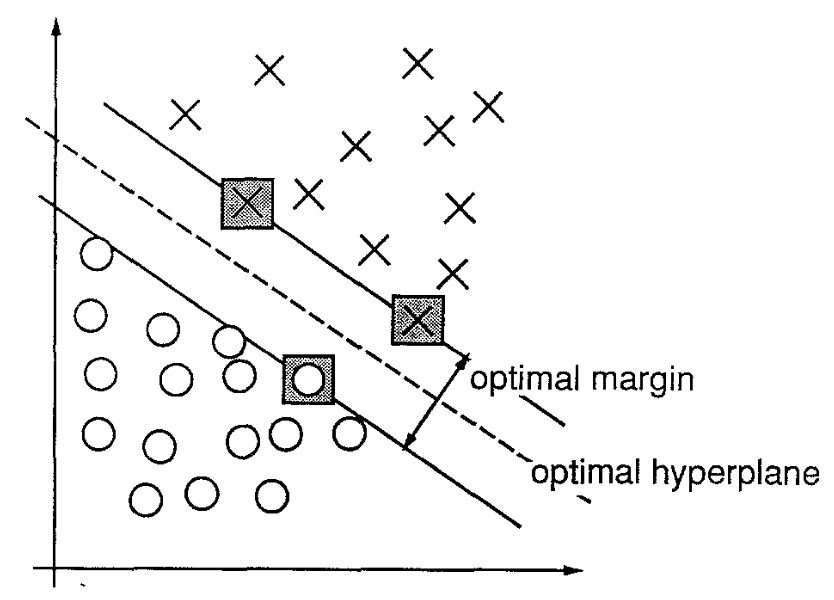
\includegraphics[width=.7\textwidth]{images/svm.png}
            \label{fig:background-optionmining-machinelearningalgorithms-svm}
        \end{figure}        
    }
}
%!TEX root = ../presentation.tex

\section{Case Study}

\begin{frame}
  \frametitle{Companies \& Keywords}

  \begin{itemize}
    \item Determined five companies
      \begin{itemize}
        \item \ford{}
        \item \gm{}
        \item \hyundai{}
        \item \toyota{}
        \item \vw{}
      \end{itemize}

    \item Determined 23 keywords/brands
  \end{itemize}
\end{frame}

\note[itemize]{
  \item Table 3.1: Keywords/Brands, page 13-15
  \begin{itemize}
    \item Ford
      \begin{itemize}
        \item Ford, Lincoln
      \end{itemize}

    \item GM
      \begin{itemize}
        \item Baojun, Buick, Cadillac, Chevrolet, GMC, Holden, Jiefang, Wuling
      \end{itemize}

    \item Hyundai
      \begin{itemize}
        \item Hyundai, KIA
      \end{itemize}

    \item Toyota
      \begin{itemize}
        \item Daihatsu, Lexus, Toyota
      \end{itemize}

    \item VW
      \begin{itemize}
        \item Audi, Bentley, Bugatti, Lamborghini, Porsche, Seat, Škoda, Volkswagen
      \end{itemize}

  \end{itemize}
  \item Table 3.2: Five Companies, page 15
}

\begin{frame}
  \frametitle{Gather Data}

  \begin{itemize}
    \item Tweets
      \begin{itemize}
        \item Using DMI-TCAT using Twitter Streaming API
        \item Gathered Tweets from \printdate{2018-02-28} and \printdate{2018-09-07}
      \end{itemize}
    
    \item Share Prices
      \begin{itemize}
        \item Yahoo Finance
      \end{itemize}
    
  \end{itemize}

\end{frame}

\note[itemize]{
  \item Why DMI-TCAT?: page 16/17
  \item Description of datasets beginning with page 24
}
%%!TEX root = ../presentation.tex

\section{Analysis}
%!TEX root = ../presentation.tex

\section{Conclusion}

\begin{frame}
    \frametitle{Detected Sentiments}

    Positive sentiment ratio by company and classifier

    {\scriptsize
  \begin{table}
      \centering
      \begin{tabular}{!l ^r ^r ^r ^r ^r}
        \hline
        & \tb{} & \nb{} & \me{} & \svm{} & Average \\ 
        \hline
            \ford{} & \SI{87.09}{\percent} & \SI{61.11}{\percent} & \SI{76.96}{\percent} & \SI{73.03}{\percent} & \SI{74.55}{\percent} \\ 
            \gm{} & \SI{90.83}{\percent} & \SI{68.60}{\percent} & \SI{80.26}{\percent} & \SI{80.45}{\percent} & \SI{80.03}{\percent} \\ 
            \hyundai{} & \SI{88.12}{\percent} & \SI{55.05}{\percent} & \SI{77.46}{\percent} & \SI{67.78}{\percent} & \SI{72.10}{\percent} \\ 
            \toyota{} & \SI{87.86}{\percent} & \SI{55.45}{\percent} & \SI{81.12}{\percent} & \SI{80.11}{\percent} & \SI{76.13}{\percent} \\ 
            \vw{} & \SI{85.20}{\percent} & \SI{47.97}{\percent} & \SI{68.26}{\percent} & \SI{64.58}{\percent} & \SI{66.50}{\percent} \\ \hline
            Average & \SI{87.82}{\percent} & \SI{57.63}{\percent} & \SI{76.81}{\percent} & \SI{73.19}{\percent} & \SI{73.86}{\percent} \\
        \hline
        \end{tabular}
    \end{table}
  }
\end{frame}

\begin{frame}
    \frametitle{Conclusion I}

    

\end{frame}
\begin{frame}[allowframebreaks]
    \frametitle{References}
    \printbibliography[title={References}]
\end{frame}
 
\end{document}